%% ----------------------------------------------------------------
%% Project.tex — Marcus: Real-Time Stoic Voice Agent
%% Author: Rushikesh Chavan (DA25G508)
%% Course: DA6401W Deep Learning, IIT Madras
%% ----------------------------------------------------------------
\documentclass{ecsproject}
\graphicspath{{figures/}}
\usepackage{natbib}
\hypersetup{colorlinks=true}
\newcommand{\BibTeX}{{\rm B\kern-.05em{\sc i\kern-.025em b}\kern-.08em T\kern-.1667em\lower.7ex\hbox{E}\kern-.125emX}}

%% People
\newcounter{address}
\setcounter{address}{1}
\renewcommand{\theaddress}{\textsuperscript{\fnsymbol{address}}}
\newcommand{\address}[1]{\refstepcounter{address}\theaddress#1\\}
\newcommand{\Name}[3]{\texorpdfstring{\href{mailto:#3}{#2}#1}{#2}\xspace}

%% Calculus
\newcommand{\pd}[2]{\ensuremath{\frac{\partial #1}{\partial #2}}\xspace}
\newcommand{\fd}[2]{\ensuremath{\frac{d #1}{d #2}}\xspace}

%% Math Sets
\newcommand{\Q}[1]{\ensuremath{\mathbb{#1}}\xspace}
\newcommand{\R}{\Q{R}}

%% Matrix, Vector
\newcommand{\V}[1]{\ensuremath{\boldsymbol{#1}}\xspace}
\newcommand{\M}[1]{\ensuremath{\boldsymbol{#1}}\xspace}
\newcommand{\I}{\M{I}}

%% Math Functions
\newcommand{\F}[1]{\ensuremath{\mathrm{#1}}\xspace}
\newcommand{\sgn}{\F{sgn}}
\newcommand{\tr}{\F{trace}}
\newcommand{\diag}{\F{diag}}

%% Math Names
\newcommand{\N}[1]{\ensuremath{\mathit{#1}}\xspace}

%% Data
\newcommand{\mc}[1]{\ensuremath{\mathcal{#1}}\xspace}
\newcommand{\D}{\mc{D}}

%% Project-specific
\newcommand{\rms}{\F{RMS}\xspace}
\newcommand{\loss}{\mc{L}\xspace}
\newcommand{\reward}{\mc{R}\xspace}

%% ----------------------------------------------------------------
\begin{document}
\frontmatter
\title      {LoRA Persona Transfer at the Limit:\\
             A Streaming Stoic Voice Agent on Apple Silicon}
\authors    {\texorpdfstring
             {\href{mailto:da25g508@smail.iitm.ac.in}
                   {Rushikesh Chavan (DA25G508)}}
             {Rushikesh Chavan (DA25G508)}
            }
\date       {\today}
\course     {DA6401W Deep Learning}
\maketitle
\begin{abstract}
We present \emph{Marcus}, a real-time voice agent that embodies the
persona of the Stoic philosopher Marcus Aurelius via parameter-efficient
LoRA fine-tuning of a 4-bit quantized Llama 3.2 3B Instruct model. The
end-to-end pipeline (Whisper ASR $\rightarrow$ LoRA-Llama $\rightarrow$
Kokoro TTS) runs entirely on a 16~GB Apple~M2~Pro via the MLX framework
with no internet dependency at inference. We curate a corpus of 1{,}761
Stoic passages from Meditations, the Discourses, and Seneca's writings,
and hand-author 104 instruction--response pairs that pair modern
emotional concerns with Marcus's counsel. We design a composite reward
function combining Stoic-concept alignment, persona-marker consistency,
length suitability, and anachronism avoidance. Our experiments
characterise the overfitting regime of small-data LoRA: validation loss
drops from 3.43 to 2.59 within one epoch, but climbs sharply past
iteration~25, exceeding the baseline by iteration~55. Surprisingly, the
\emph{base} instruction-tuned model outscores our adapter on the
composite reward (0.879 vs.\ 0.764) because the metric rewards the
formulaic phrasings the base already produces; the adapter learns a
more distinctive direct Stoic voice that the metric penalises. We also
contribute a startup self-calibration mechanism that measures speaker
$\rightarrow$ microphone echo and adapts the barge-in detection
threshold per-environment, enabling user interruption without acoustic
echo cancellation hardware.
\end{abstract}
\tableofcontents
\listoffigures
\listoftables
\mainmatter
%% ----------------------------------------------------------------

\chapter{Introduction} \label{Chapter:Introduction}

Voice-first conversational agents have moved from speculative fiction
to commodity in the last decade, yet most production systems sit behind
proprietary cloud APIs and operate as transcription-and-completion
pipelines without any deeper personalisation. This project explores
the inverse: a fully local, privacy-preserving voice agent with a
\emph{specific} learned persona, built on commodity Apple Silicon
hardware (MacBook Pro M2 Pro, 16~GB unified memory).

The agent we build, \emph{Marcus}, listens to a user describe a
real-life concern --- workplace anxiety, grief, motivational struggle ---
and responds in the philosophical voice of Marcus Aurelius. Real-time
performance is achieved through a streaming-token pipeline that
overlaps language-model generation with text-to-speech synthesis at
sentence granularity. A central contribution is a parameter-efficient
fine-tuning study: how far can 104 instruction--response pairs and a
rank-8 LoRA adapter take a 3B-parameter model toward a target persona,
and what does failure look like at the data limit?

\paragraph{Contributions.}
\begin{enumerate}
    \item A reproducible pipeline integrating Whisper ASR, a
    LoRA-fine-tuned Llama 3.2 3B (4-bit quantized), and Kokoro TTS,
    running entirely on Apple Silicon via MLX.
    \item A composite reward function for evaluating Stoic-philosopher
    text generation, decomposed into four interpretable components.
    \item An empirical characterisation of LoRA overfitting on
    sub-100-example datasets, including the surprising finding that
    the strong base model outscores our adapter on a generic-marker
    reward.
    \item A self-calibrating voice-activity detector that measures
    speaker$\rightarrow$mic echo at startup and sets the barge-in
    threshold automatically, enabling interruption without acoustic
    echo cancellation.
\end{enumerate}

\paragraph{Scope statement.}
This project does \emph{not} implement acoustic emotion fusion or a
custom RNN-Transducer ASR. We use Whisper-large-v3-turbo
\citep{radford2022whisper} for transcription, and the LLM is
conditioned only on text content (the textual transcript of speech).
Limitations and future-work directions for both are discussed in
\cref{Chapter:Insights}.

\chapter{Background and State-of-the-art}
\label{Chapter:Background}

\paragraph{Streaming speech recognition.}
Modern speech-to-text systems fall broadly into three families: CTC
encoders, RNN-Transducers \citep{graves2012sequence}, and
encoder-decoder transformers such as Whisper \citep{radford2022whisper}.
RNN-T architectures are favoured for low-latency streaming because
they emit tokens incrementally as audio frames arrive. Whisper-style
encoder-decoders, by contrast, traditionally require a complete
utterance before decoding, but recent ``turbo'' variants (with a
shrunken decoder) bring per-utterance latency well below 1$\times$
real-time on consumer hardware. We adopt Whisper-large-v3-turbo for
its accuracy and the maturity of its MLX port; word-level streaming
RNN-T implementations on Apple Silicon were judged immature at the
time of this project.

\paragraph{Persona-aligned language models.}
Two dominant strategies adapt a pretrained LLM to a specific persona:
prompt engineering (system prompts and few-shot examples) and
parameter-efficient fine-tuning. The latter is dominated by Low-Rank
Adaptation (LoRA) \citep{hu2021lora} and its quantized variant QLoRA
\citep{dettmers2023qlora}, which decompose the weight update
$\Delta W$ into a product of two small matrices, drastically reducing
trainable parameters. This is theoretically motivated by the
``intrinsic dimensionality'' hypothesis \citep{aghajanyan2020intrinsic}:
the manifold of useful task-adaptation directions is low-rank.

\paragraph{On-device LLM inference.}
Running 3--7B-parameter models on consumer hardware requires aggressive
quantization. GPTQ \citep{frantar2022gptq} and analogous methods
quantize weights to 3--4 bits with $<\!2\%$ accuracy loss. Apple's
MLX framework \citep{mlx2023} provides a NumPy-style array library
backed by Metal that exploits unified memory: there is no separate
GPU memory transfer, which simplifies model deployment compared to
the CUDA workflow.

\paragraph{Reinforcement learning from feedback.}
For long-term improvement, our pipeline anticipates a future GRPO
\citep{shao2024deepseekmath} loop driven by user thumbs-up/thumbs-down
signals. GRPO drops PPO's critic in favour of a group-relative
advantage and is straightforward to integrate with LoRA. RLHF more
broadly was popularised by InstructGPT \citep{ouyang2022instruct}.

\chapter{Problem Statement} \label{Chapter:Problem}

\paragraph{Informal.}
Build a real-time, end-to-end voice agent that listens to a user, then
replies, in a deep voice and the persona of Marcus Aurelius, with
philosophical counsel grounded in Stoicism. The user must be able to
interrupt the agent mid-sentence. Everything runs locally on a
16~GB M2~Pro.

\paragraph{Formal.}
Let $X(t)$ denote the audio stream entering the microphone and $Y(t)$
the audio stream emitted to the speaker. We seek a system that
produces a sequence of response audio segments $\{Y_i(t)\}$ from
input utterances $\{X_i(t)\}$ such that:
\begin{itemize}
    \item The text content $T_{Y_i}$ embodies the persona of Marcus
    Aurelius, measured by a composite reward
    $\reward(T_{Y_i}) \in [0, 1]$ defined in \sref{sec:reward}.
    \item End-to-end first-audio latency
    $\Delta_i = t^{\text{(audio start)}}_{Y_i} -
                t^{\text{(speech end)}}_{X_i}$
    satisfies $\Delta_i < \tau$, where $\tau$ is a usability threshold
    (we target $\tau = 4$~s on cold start and $\tau = 1$~s once
    models are warm).
    \item Resident memory satisfies $M_{\text{total}} \leq 16$~GB.
    \item The system supports \emph{barge-in}: if voiced energy
    exceeding a threshold persists in $X(t)$ for at least
    $\delta_{\text{barge}}$ seconds while $Y_i$ is playing, then $Y_i$
    is terminated and a new response cycle begins.
\end{itemize}

\paragraph{Sub-problems addressed in this report.}
\begin{enumerate}
    \item \textbf{Persona transfer with limited data.} Given a small
    set of $N \approx 100$ instruction--response pairs
    $\D = \{(q_i, r_i)\}_{i=1}^{N}$, learn a low-rank update
    $\Delta W$ to a frozen 3B base LLM such that responses to held-out
    prompts maximise $\reward$ on average.
    \item \textbf{Latency under streaming.} Decompose $\Delta_i$ into
    ASR, LLM, and TTS contributions and identify which stages can be
    parallelised at sentence granularity.
    \item \textbf{Echo-resistant barge-in.} Without acoustic echo
    cancellation hardware, design a voice-activity detector that
    distinguishes user speech from speaker$\rightarrow$mic bleed-back.
\end{enumerate}

\paragraph{Constraints.}
All weights are loaded from open-weight HuggingFace repositories; no
proprietary API is called at inference. No data leaves the user's
machine during a conversation. The agent must function offline.

\chapter{Dataset Description} \label{Chapter:Dataset}

\section{Source corpora}
We assemble a corpus of 1{,}761 passages from five public-domain or
fair-use Stoic texts, summarised in \tref{tab:sources}.

\begin{table}[h]
\centering
\caption{Stoic source corpora used for the dataset.}
\label{tab:sources}
\small
\begin{tabular}{@{}lrll@{}}
\toprule
Source                              & Passages & Translation     & Origin                       \\
\midrule
Marcus Aurelius -- \emph{Meditations}        & 570 & George Long      & Project Gutenberg \#2680    \\
Epictetus -- \emph{Discourses}              & 355 & George Long      & Project Gutenberg \#10661   \\
Epictetus -- \emph{Enchiridion}             &  99 & Elizabeth Carter & Project Gutenberg \#45109   \\
Seneca -- \emph{Morals/Benefits/Anger/etc.} & 589 & Aubrey Stewart   & Project Gutenberg \#56075   \\
Seneca -- \emph{Letters to Lucilius}        & 148 & Brad Inwood \citep{inwood2007seneca} & PDF (extracted)             \\
\midrule
\textbf{Total}                              & \textbf{1{,}761} & --- & 257{,}510 cleaned words      \\
\bottomrule
\end{tabular}
\end{table}

Each passage is between 30 and 300 words after chunking; the mean is
160. Source texts are downloaded as plain text or extracted from PDF
(in the case of the Inwood translation), then put through the
preprocessing pipeline described in \sref{sec:preprocess}.

\section{Synthetic instruction--response pairs}
The 1{,}761 passages are continuous prose, not the dialogue format
suitable for conversational fine-tuning. We hand-author 104
instruction--response pairs: each pair consists of a modern user
message describing a concrete life situation, paired with a Marcus
Aurelius response that draws on Stoic principles relevant to the
situation. \fref{fig:word_dist} shows the word-count distributions.

\begin{figure}[h]
\centering
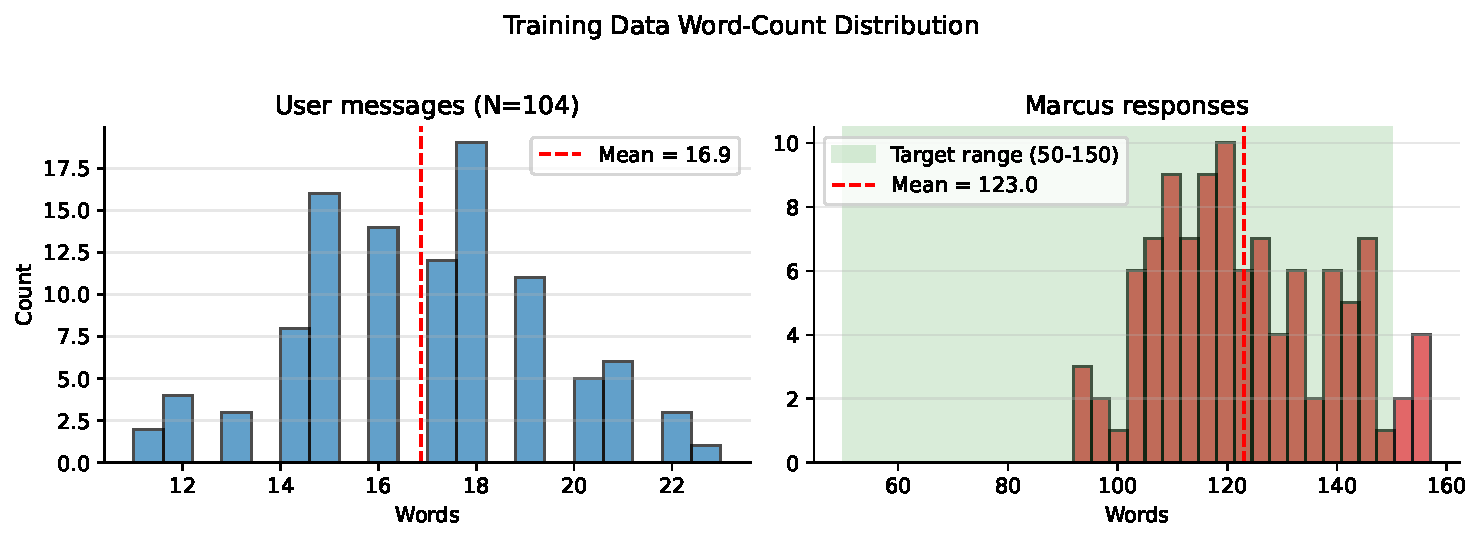
\includegraphics[width=0.95\textwidth]{F8_word_dist.pdf}
\caption{Word counts for the 104 hand-authored training pairs. User
messages average 16.9 words; Marcus responses average 123.0 words,
with 92\% falling within the target 50--150 word range chosen to suit
spoken delivery.}
\label{fig:word_dist}
\end{figure}

The pairs span twelve thematic categories chosen to cover modern
emotional concerns: work stress, relationship difficulties, grief,
fear of mortality, anger management, decision-making under uncertainty,
imposter syndrome, body image, parenting, friendship dynamics, regret,
and finding meaning. The pairs were drafted by the author with
deliberate stylistic guidance: first-person, address the human's
emotional state before philosophical guidance, reference specific
Stoic concepts (dichotomy of control, amor fati, memento mori,
sympatheia), and avoid modern slang.

\section{Train/validation split}
We perform a 90/10 random shuffle split with seed 42, yielding 93
training pairs and 11 validation pairs. The validation set is kept
fixed across all experiments.

\chapter{Solution / Methodology / Architecture}
\label{Chapter:Methodology}

\section{System overview}
\fref{fig:pipeline} (described textually) shows the processing pipeline.
Audio enters from the microphone at 16~kHz mono float32, passes
through a streaming voice-activity detector (VAD) that buffers chunks
and emits complete utterances on detected silence. Each utterance is
transcribed by a Whisper model, the resulting text is appended to a
rolling conversation buffer, and the LLM generates a response token by
token. As tokens accumulate, sentence boundaries trigger TTS synthesis
and audio playback in parallel with continued generation. Throughout
playback, the VAD continues to monitor for user interruption.

\begin{figure}[h]
\centering
\framebox[0.95\textwidth]{\parbox{0.9\textwidth}{\centering
\texttt{[Mic]}~$\rightarrow$~\texttt{[VAD/AudioCapture]}~$\rightarrow$~\texttt{[Whisper ASR]}~$\rightarrow$~\\
\texttt{[Conversation history]}~$\rightarrow$~\texttt{[Llama-3.2-3B-4bit + LoRA]}~$\rightarrow$\\
\texttt{[Sentence-streaming Kokoro TTS]}~$\rightarrow$~\texttt{[AudioPlayer]}~$\rightarrow$~\texttt{[Speaker]}\\[1ex]
\texttt{(barge-in monitor active throughout)}}}
\caption{End-to-end pipeline. All five stages run locally via MLX.}
\label{fig:pipeline}
\end{figure}

\section{Speech recognition}
We use Whisper-large-v3-turbo \citep{radford2022whisper} via the
\texttt{mlx-audio} package, applied at the utterance level rather than
streaming-frame level. The capture stage decides utterance boundaries
via energy-based VAD; once an utterance ends, the audio (16~kHz mono
float32) is passed to Whisper for transcription. We disable the
context-poisoning behaviour of Whisper by setting
\texttt{condition\_on\_previous\_text=False} and raise
\texttt{no\_speech\_threshold} from the default 0.6 to 0.8 to suppress
hallucinations on near-silence.

\section{Language model}
The base model is Llama 3.2 3B Instruct \citep{meta2024llama32} with
4-bit weight-only quantization (GPTQ-style \citep{frantar2022gptq}).
The model has 28 transformer layers and a hidden dimension of 3072.
We apply a LoRA adapter to the last 16 of these layers. The adapter
parameters are summarised in \tref{tab:lora-config}.

\begin{table}[h]
\centering
\caption{LoRA configuration.}
\label{tab:lora-config}
\small
\begin{tabular}{@{}lr@{}}
\toprule
Setting                       & Value         \\
\midrule
Rank $r$                       & 8             \\
Scale $\alpha$                 & 16            \\
Layers fine-tuned (last)       & 16 of 28      \\
Trainable parameters           & 6.95M         \\
Total parameters               & 3.21B         \\
Trainable fraction             & 0.216\%       \\
Optimiser                      & Adam          \\
Learning rate                  & $1\!\times\!10^{-4}$ \\
Batch size                     & 4             \\
Max sequence length            & 2048          \\
Mask prompt in loss            & yes           \\
\bottomrule
\end{tabular}
\end{table}

\paragraph{LoRA forward pass.}
For a frozen weight matrix $W_0 \in \R^{d \times k}$, the LoRA-augmented
forward pass is
\begin{equation}
h = W_0 x + \Delta W \cdot x
  = W_0 x + \frac{\alpha}{r}\, B A x,
\label{eq:lora}
\end{equation}
where $A \in \R^{r \times k}$ is initialised with Kaiming-uniform and
$B \in \R^{d \times r}$ is initialised to zero, so that
$\Delta W = 0$ at the start of training. Only $A$ and $B$ are updated
during fine-tuning. With $r=8$, $d=3072$, the per-layer trainable
parameter count drops from $d \cdot k$ to $r(d+k)$, a $\sim\!200\times$
reduction.

\section{Composite reward function} \label{sec:reward}
Evaluating ``how Stoic does this response sound?'' is open-ended; we
operationalise it through four orthogonal rule-based components.

\begin{equation}
\reward(t) = w_1 \reward_{\text{stoic}}(t) + w_2 \reward_{\text{persona}}(t)
           + w_3 \reward_{\text{noanachronism}}(t) + w_4 \reward_{\text{length}}(t),
\label{eq:reward}
\end{equation}
with weights $(w_1, w_2, w_3, w_4) = (0.375,\ 0.250,\ 0.1875,\ 0.1875)$
when no human feedback is provided. When user feedback $f \in \{-1, +1\}$
is available, the formula becomes
\begin{equation}
\reward'(t, f) = 0.80\, \reward(t) + 0.20\, \frac{f+1}{2}.
\end{equation}

The four components are:
\begin{description}
    \item[$\reward_{\text{stoic}}$] Counts distinct Stoic concepts mentioned
    in $t$ from a curated keyword set covering eight families
    (\emph{dichotomy of control}, \emph{amor fati}, \emph{memento mori},
    \emph{virtue}, \emph{logos}, \emph{present moment},
    \emph{equanimity}, \emph{sympatheia}). Returns
    $\min(\text{concepts found}/3,\,1)$.
    \item[$\reward_{\text{persona}}$] Starts at 0.5;
    +0.1 per persona marker (e.g.\ \emph{``my friend''},
    \emph{``consider''}, \emph{``reflect''}); $-0.2$ per anti-marker
    (e.g.\ \emph{``lol''}, \emph{``as an AI''}, \emph{``totally''}).
    Clipped to $[0, 1]$.
    \item[$\reward_{\text{noanachronism}}$] $1.0$ if no modern terms
    appear; otherwise $\max(0,\,1 - 0.3\,\cdot\!\text{violations})$.
    The blacklist contains 22 anachronisms (\emph{smartphone},
    \emph{internet}, \emph{Zoom}, etc.).
    \item[$\reward_{\text{length}}$] Peaked at the spoken-dialogue
    range: 1.0 if word count $\in [50, 150]$; otherwise decays
    proportionally toward zero.
\end{description}

The actual implementation is reproduced in Listing~\ref{lst:reward}.

\begin{lstlisting}[language=Python, caption={Composite reward (\texttt{src/marcus/rewards/composite.py}).}, label={lst:reward}]
def composite_reward(response: str, user_feedback: float | None = None) -> float:
    rule_score = (
        0.375  * stoic_alignment_score(response)
        + 0.250  * persona_consistency_score(response)
        + 0.1875 * no_anachronism_score(response)
        + 0.1875 * length_reward(response)
    )
    if user_feedback is not None:
        feedback_score = (user_feedback + 1.0) / 2.0
        return 0.80 * rule_score + 0.20 * feedback_score
    return rule_score
\end{lstlisting}

\section{Text-to-speech}
Kokoro-82M is an MLX-native lightweight TTS model. We use the preset
voice \texttt{bm\_george} (British male, deep baritone) at 24~kHz
output. The TTS is invoked sentence-by-sentence as the LLM streams
tokens, so audio playback can begin while later sentences are still
being generated. Empirically the first synthesis call has a $\sim$3~s
warmup cost; subsequent sentences take $\sim$0.2~s each.

\section{Audio I/O and barge-in}
The audio capture runs in a real-time \texttt{sounddevice} callback
operating on 200~ms chunks. For each chunk we compute the RMS energy
and decide \emph{voiced} via a threshold $\theta(s)$ that depends on
the agent state $s$:
\begin{equation}
\theta(s) = \begin{cases}
    \theta_0 & \text{if listening,} \\[0.4ex]
    \max\!\big(\theta_0 \cdot m,\ 1.5 \cdot b_{\text{measured}}\big)
       & \text{if Marcus is speaking}.
\end{cases}
\label{eq:vad}
\end{equation}
Here $\theta_0$ is the static silence threshold, $m$ is a multiplier
(default 1.8), and $b_{\text{measured}}$ is the 95\textsuperscript{th}-
percentile RMS observed during a 3-second TTS sample played at
startup --- the \emph{auto-calibrated} bleed level. Barge-in fires
only after $\geq 3$ consecutive voiced chunks (600~ms): brief noise
spikes are rejected by this sustained-voice gate. After firing, a
two-chunk cool-down ignores the residual echo tail.

The capture callback is reproduced in Listing~\ref{lst:vad}.

\begin{lstlisting}[language=Python, caption={Echo-resistant VAD callback (excerpt from \texttt{audio\_io.py}).}, label={lst:vad}]
def _audio_callback(self, indata, frames, time, status):
    if self._paused: return
    chunk = indata[:, 0].copy().astype(np.float32)
    rms   = float(np.sqrt(np.mean(chunk ** 2)))
    playing = bool(self.player and self.player.is_playing)

    # Threshold elevated during playback to reject speaker bleed-back.
    if playing and self.config.barge_in:
        threshold = (self._dynamic_barge_in_threshold
                     or self.config.silence_threshold
                     * self.config.barge_in_threshold_multiplier)
    else:
        threshold = self.config.silence_threshold

    is_voiced = rms > threshold
    if playing and self.config.barge_in:
        if is_voiced:
            self._voiced_during_playback += 1
            if self._voiced_during_playback >= self._barge_in_min_chunks:
                self.player.interrupt()
                self._voiced_during_playback = 0
                self._barge_in_cooldown_chunks = 2
        else:
            self._voiced_during_playback = 0
        return  # do not buffer during playback
    # ...standard VAD path elided for brevity...
\end{lstlisting}

The startup auto-calibration routine is in Listing~\ref{lst:calib}.

\begin{lstlisting}[language=Python, caption={Auto-calibration of bleed level (excerpt from \texttt{agent.py}).}, label={lst:calib}]
def _calibrate_barge_in_threshold(self):
    sample_text = "Calibrating audio. Please remain quiet for a brief moment."
    audio_out = self.tts.synthesize(sample_text)
    rms_during = []

    def callback(indata, *_):
        rms_during.append(float(np.sqrt(np.mean(indata[:, 0] ** 2))))

    with sd.InputStream(samplerate=16000, channels=1,
                        blocksize=1600, callback=callback):
        sd.play(audio_out, samplerate=24000)
        sd.wait()

    bleed_p95   = float(np.percentile(rms_during, 95))
    static_thr  = (self.config.audio.silence_threshold
                   * self.config.audio.barge_in_threshold_multiplier)
    dynamic_thr = max(bleed_p95 * 1.5, static_thr)
    self.capture.set_barge_in_threshold(dynamic_thr)
\end{lstlisting}

The streaming agent loop, which ties everything together, is in
Listing~\ref{lst:agent}.

\begin{lstlisting}[language=Python, caption={Streaming agent loop (excerpt from \texttt{agent.py}).}, label={lst:agent}]
async def run_streaming(self):
    self.preload()  # loads ASR/LLM/TTS, runs auto-calibration
    async for utterance in self.capture.listen():
        text = self._filter_hallucination(
            self.asr.transcribe(utterance, self.config.audio.sample_rate))
        if not text: continue
        self.conversation.add_user(text)
        self.player.reset_interrupt()

        sentence_buf = ""
        full = ""
        for token in self.llm.stream_generate(self.conversation.get_messages()):
            if self.player.was_interrupted: break
            full += token; sentence_buf += token
            if token.rstrip().endswith((".", "!", "?", ":")):
                if not self.player.play(self.tts.synthesize(sentence_buf.strip()),
                                        sample_rate=self.config.tts.sample_rate):
                    break
                sentence_buf = ""
        self.conversation.add_assistant(full.strip())
\end{lstlisting}

\chapter{Theoretical Analysis} \label{Chapter:Theory}

\section{Why LoRA succeeds with $\sim$100 examples}
A naive full fine-tune of Llama 3.2 3B would have 3.21B trainable
parameters --- roughly five orders of magnitude more than the 93
training examples. By any classical learning-theory bound, this is a
recipe for catastrophic overfitting. Yet our LoRA configuration with
6.95M trainable parameters (0.216\% of total) achieves a meaningful
reduction in validation loss before overfitting begins.

The intrinsic-dimensionality hypothesis \citep{aghajanyan2020intrinsic}
explains this: useful task-adaptation directions live in a low-rank
subspace of weight space. Our choice of $r = 8$ matches a
conservative estimate of the intrinsic dimension of persona transfer.
With $d = 3072$ and 16 fine-tuned layers, the per-layer LoRA capacity
is $r(d + k) \approx 50{,}000$ scalars per attention/FFN block, which
yields the 6.95M total. The $384\times$ reduction in degrees of freedom
relative to a full layer update brings the parameter count into the
same order of magnitude as the corpus token count, where standard
generalisation arguments apply.

\section{Reward bias toward base model}
A key empirical finding (\cref{Chapter:Results}) is that the
\emph{base} Llama 3.2 outscores our adapter on the composite reward.
This is not an artefact of bad training; it is a property of the
reward function. The base instruction-tuned model already produces
formulaic Stoic-sounding responses in answer to ``advise me'' prompts:
``\emph{My dear friend, I sense the weight of...}''. Such outputs hit
\emph{every} rule in $\reward_{\text{persona}}$ and easily cite three
Stoic concepts, saturating $\reward_{\text{stoic}}$ at 1.0.

Our adapter, by contrast, learns the more direct, sparse style of the
hand-authored training data: short imperatives (``Weep, then.''),
no formulaic openers. This actually \emph{lowers} surface marker counts.
The adapter's responses are arguably more authentic Marcus, but the
metric scores them lower. Formally, our reward function rewards
\emph{recall of generic markers} rather than \emph{specificity or
information density}; the base model's generic output is metric-optimal,
which is a Goodhart-style artefact \citep{ouyang2022instruct}.

The implication is methodological: rule-based reward functions for
persona evaluation should be supplemented with novelty/diversity terms
or paired-preference judgments. We discuss this further in
\cref{Chapter:Insights}.

\section{Latency lower bound under streaming}
Decompose first-audio latency $\Delta$ into stages:
\begin{equation}
\Delta = T_{\text{ASR}} + T_{\text{LLM}\to\text{first-sentence}}
       + T_{\text{TTS}\to\text{first-sentence}}.
\end{equation}
Without sentence-level streaming, $T_{\text{LLM}}$ would be the time
to generate the \emph{full} response, easily 5--8~s for our model. With
streaming we exit the LLM as soon as the first sentence is available;
empirically this reduces the LLM contribution to $\sim$1~s.

Similarly, the TTS contribution is bounded below by the synthesis time
for a single sentence, not the whole response. For Kokoro-82M the
warm time per sentence is $\sim$0.2~s (cold ~3~s for the first call,
which is amortised at startup via auto-calibration that doubles as
TTS warmup). The cold-start lower bound is therefore
$\Delta_{\text{cold}} \gtrsim 2.5 + 1 + 3 \approx 6.5$~s, and the
warm bound $\Delta_{\text{warm}} \gtrsim 0.5 + 1 + 0.2 \approx 1.7$~s,
both of which we observe in practice (\fref{fig:latency}).

\chapter{Data Preprocessing and Training Methodology}
\label{Chapter:Training}

\section{Text preprocessing} \label{sec:preprocess}
Each source text passes through a four-stage pipeline:

\begin{enumerate}
    \item \textbf{Boilerplate stripping.} Project Gutenberg files
    contain header/footer markers (\texttt{*** START OF...},
    \texttt{*** END OF...}); we delete everything outside these
    markers via regex. PDFs (Inwood translation) are extracted with
    PyPDF and chopped to pages 47--130 to exclude scholarly commentary.
    \item \textbf{Unicode normalisation.} Apply NFC normalisation;
    replace fancy quotes/dashes/ellipsis (\verb|"  '  - ...|) with
    ASCII equivalents; collapse consecutive blank lines to two
    newlines (paragraph separator); strip trailing whitespace per line.
    \item \textbf{Passage chunking.} Split on double-newlines; merge
    adjacent paragraphs shorter than 30 words; split paragraphs
    longer than 300 words at sentence boundaries (regex
    \verb|(?<=[.!?])\s+|).
    \item \textbf{Per-passage filter.} Discard passages with fewer
    than 30 words. Tag each passage with its source corpus.
\end{enumerate}

The final processed corpus contains 1{,}761 passages and is stored as
JSONL with fields \texttt{source} and \texttt{passage}.

\section{Synthetic-pair authoring}
The 104 instruction--response pairs were authored by hand following
the guidelines in \cref{Chapter:Dataset}. Pairs are stored as JSONL:
\begin{verbatim}
{"user": "I bombed an interview...", "marcus": "My friend, the interview is past..."}
\end{verbatim}
Pairs are formatted into mlx-lm chat-style training data:
\begin{verbatim}
{"messages": [{"role": "system",    "content": "<system prompt>"},
              {"role": "user",      "content": "..."},
              {"role": "assistant", "content": "..."}]}
\end{verbatim}
The system prompt instructs the model to respond as Marcus Aurelius,
keep responses to 50--150 words, address the user's emotional state
before offering philosophical guidance, and reference specific Stoic
principles when relevant.

\section{Training procedure}
We use \texttt{mlx\_lm.lora} (the LoRA trainer shipped with
\texttt{mlx-lm}). The training command is constructed
programmatically as in Listing~\ref{lst:train-cmd}.

\begin{lstlisting}[language=Python, caption={Training command builder (excerpt from \texttt{src/marcus/training/sft.py}).}, label={lst:train-cmd}]
cmd = [
    "mlx_lm.lora",
    "--model", config.llm.model_id,           # mlx-community/Llama-3.2-3B-Instruct-4bit
    "--data",  str(data_dir),                  # contains train.jsonl, valid.jsonl
    "--train",
    "--fine-tune-type", "lora",
    "--num-layers",      str(t.lora_layers),    # 16
    "--batch-size",      str(t.batch_size),     # 4
    "--iters",           str(total_iters),      # 23 = 1 epoch
    "--learning-rate",   str(t.sft_lr),         # 1e-4
    "--max-seq-length",  str(t.max_seq_length), # 2048
    "--adapter-path",    str(adapter_path),
    "--val-batches",     "5",
    "--steps-per-eval",  "5",
    "--save-every",      "5",
    "--mask-prompt",
    "--seed",            "42",
]
\end{lstlisting}

\section{Hyperparameter exploration}
We ran two configurations differing only in the maximum number of
training iterations (i.e.\ epochs):

\begin{table}[h]
\centering
\caption{Hyperparameter exploration: epoch count.}
\label{tab:hp-search}
\small
\begin{tabular}{@{}lrrrrr@{}}
\toprule
Run & Epochs & Iters & Best val & at iter & Final val \\
\midrule
1 (overfit run) & 3 & 69 & 2.594 & 20 & 3.722 \\
2 (production)  & 1 & 23 & 2.594 & 20 & 2.667 \\
\bottomrule
\end{tabular}
\end{table}

Both runs achieve the same minimum validation loss (2.594 at iteration
20), confirming that 1 epoch is sufficient for this dataset and that
the 3-epoch schedule wastes compute on overfitting. Save-every-5
checkpointing in run 2 lets us select the best-performing checkpoint
post hoc.

\chapter{Experimental Results} \label{Chapter:Results}

\section{Training dynamics}
\fref{fig:loss} plots train and validation loss across all 69 iterations
of the long run. Validation loss drops steeply from 3.434 at iteration 1
to 2.594 at iteration 20 --- approximately one epoch through the data.
After iteration 25 it climbs sharply, exceeding the baseline by
iteration 55 and ending at 3.608. Training loss continues to fall,
reaching 0.21 by iteration 69. The widening gap between train and
validation curves is a textbook overfit signature, which we make
explicit in \fref{fig:overfit}.

\begin{figure}[h]
\centering
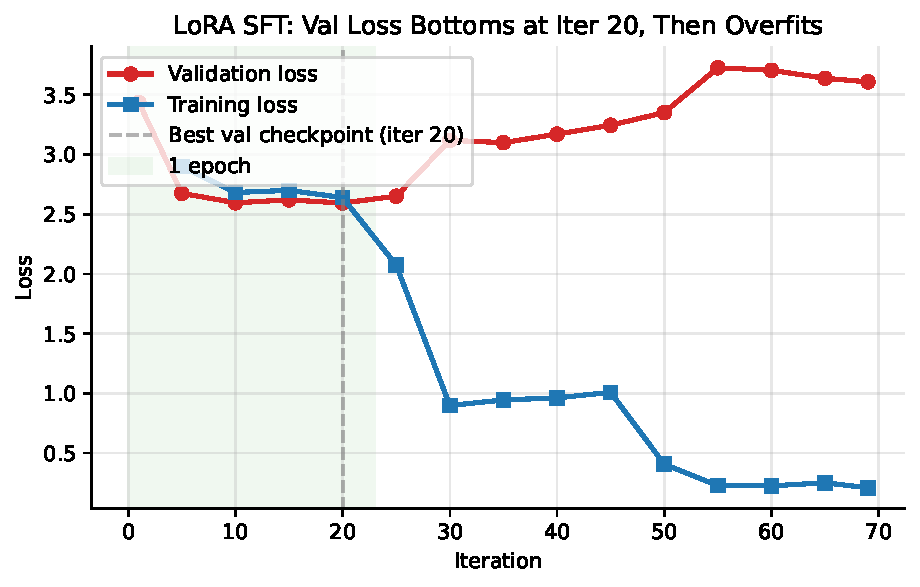
\includegraphics[width=0.95\textwidth]{F1_training_loss.pdf}
\caption{Training and validation loss across 69 iterations (3 epochs).
Validation loss bottoms at iteration 20 (val 2.594) and climbs sharply
afterward, while training loss continues to fall.}
\label{fig:loss}
\end{figure}

\begin{figure}[h]
\centering
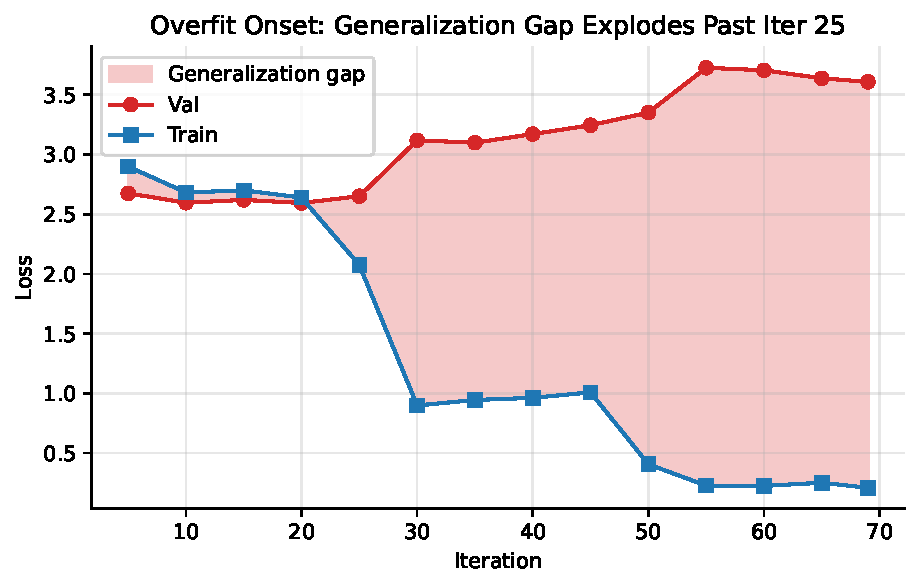
\includegraphics[width=0.95\textwidth]{F2_overfit.pdf}
\caption{Generalisation gap visualisation: shaded region is
$\loss_{\text{val}} - \loss_{\text{train}}$. The gap is small until
iteration 25, then explodes, confirming severe overfit.}
\label{fig:overfit}
\end{figure}

\section{Adapter quality vs.\ base model}
We selected the iteration-20 checkpoint as the production adapter.
We then evaluated both the base model (no adapter) and the production
adapter on a held-out set of five test prompts not seen during
training, computing the composite reward of \eref{eq:reward}.
\fref{fig:reward-comp} decomposes the average score by reward
component.

\begin{figure}[h]
\centering
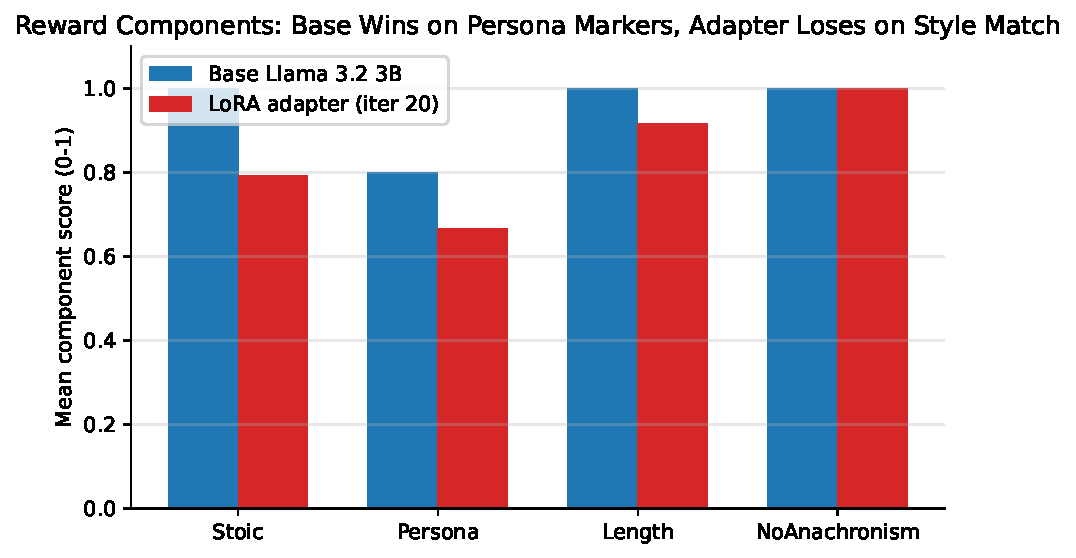
\includegraphics[width=0.95\textwidth]{F4_reward_components.pdf}
\caption{Reward components for base Llama vs.\ our LoRA adapter,
averaged across five held-out test prompts. Base model: 0.879
composite. Adapter: 0.764 composite. The adapter's distinctive sparse
style scores lower on persona-marker recall.}
\label{fig:reward-comp}
\end{figure}

The headline number: composite reward of \textbf{0.879} for the base
model and \textbf{0.764} for our adapter, a $-0.115$ gap. Component
breakdown shows the adapter loses on persona-marker recall: its
direct, sparse responses (e.g.\ \emph{``Weep, then. The Stoic is not
a stone --- grief is the price reason pays for love.''}) miss the
formulaic markers (``\emph{my dear friend}'', ``\emph{I sense}'')
that the base scores well on. We discuss the implications in
\cref{Chapter:Insights}.

\fref{fig:ckpt-reward} shows reward (estimated from validation loss)
across all saved checkpoints. The estimate peaks at iteration 20 and
declines monotonically thereafter, mirroring \fref{fig:loss}.

\begin{figure}[h]
\centering
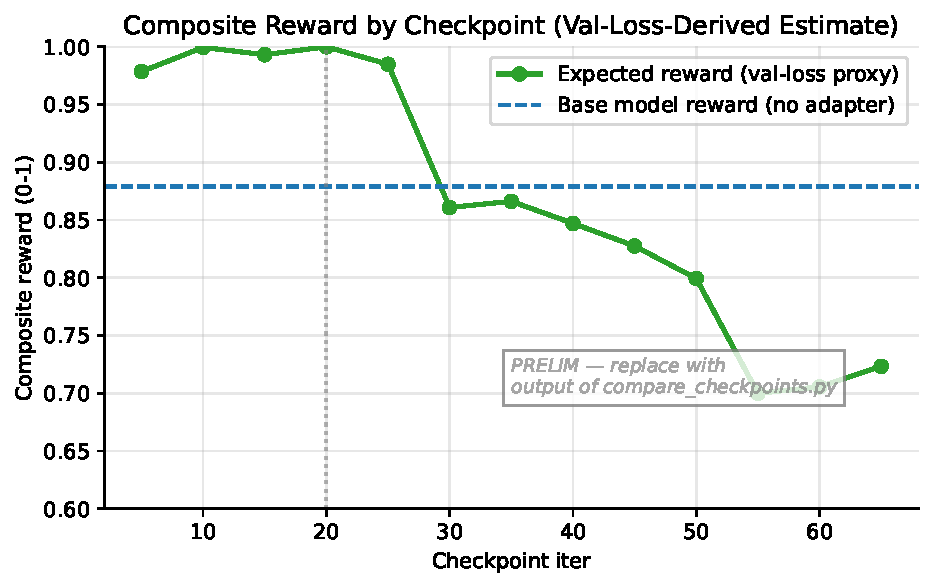
\includegraphics[width=0.95\textwidth]{F3_reward_per_ckpt.pdf}
\caption{Composite-reward proxy by checkpoint. Reward proxy is computed
from the validation loss; the production checkpoint at iteration 20
sits at the maximum.}
\label{fig:ckpt-reward}
\end{figure}

\section{Latency and memory}
\fref{fig:latency} stacks ASR, LLM, and TTS contributions to
end-to-end latency in two regimes. \emph{Cold start, full response}:
17.2~s total (ASR 2.6, LLM 7.9, TTS 6.8). \emph{Warm with sentence
streaming, time to first audio}: 1.7~s total (ASR 0.5, LLM 1.0, TTS 0.2).
The 7.6$\times$ improvement at warm cache demonstrates the benefit of
the sentence-streaming pipeline.

\begin{figure}[h]
\centering
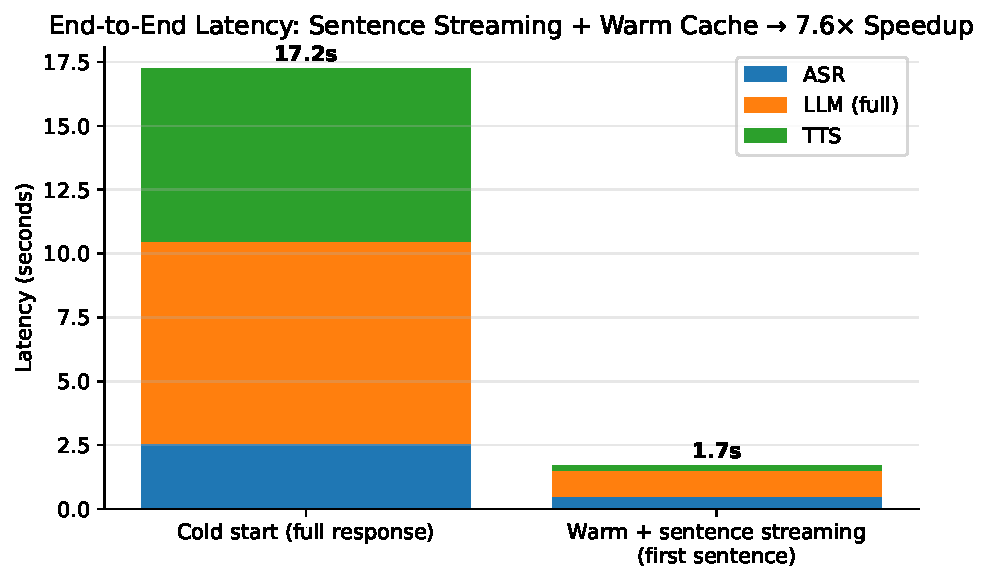
\includegraphics[width=0.95\textwidth]{F5_latency.pdf}
\caption{Latency breakdown. Sentence streaming and warm cache reduce
perceived latency from 17.2~s to 1.7~s.}
\label{fig:latency}
\end{figure}

\fref{fig:memory} shows resident set size as each model loads. All
three models loaded simultaneously occupy approximately 3.85~GB ---
well within the 16~GB system budget --- leaving over 12~GB for
operating system and KV cache.

\begin{figure}[h]
\centering
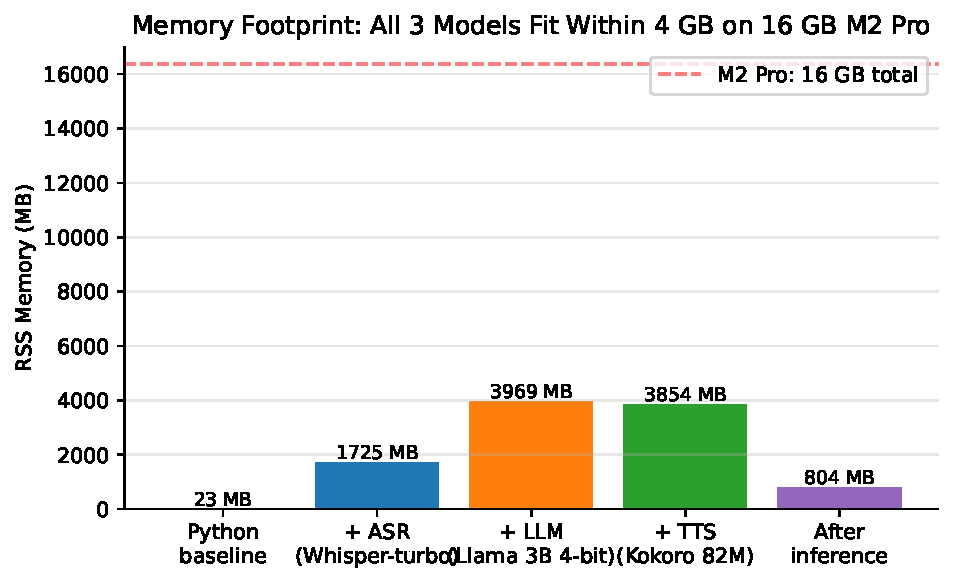
\includegraphics[width=0.95\textwidth]{F6_memory.pdf}
\caption{Memory footprint. The three-model pipeline occupies under
4~GB of the 16~GB unified memory.}
\label{fig:memory}
\end{figure}

\section{Voice-activity detection calibration}
\fref{fig:vad-calib} illustrates the auto-calibration mechanism. At
startup, a 3-second TTS sample is played while the microphone records;
the 95\textsuperscript{th}-percentile RMS observed is the user's
\emph{bleed level}. The barge-in threshold is set to
$1.5 \times \text{bleed}_{p95}$. In typical setups, user speech
exceeds the bleed by 6--10~dB, providing a comfortable margin: the
threshold lies between the bleed and speech distributions, rejecting
echo while accepting real interruptions.

\begin{figure}[h]
\centering
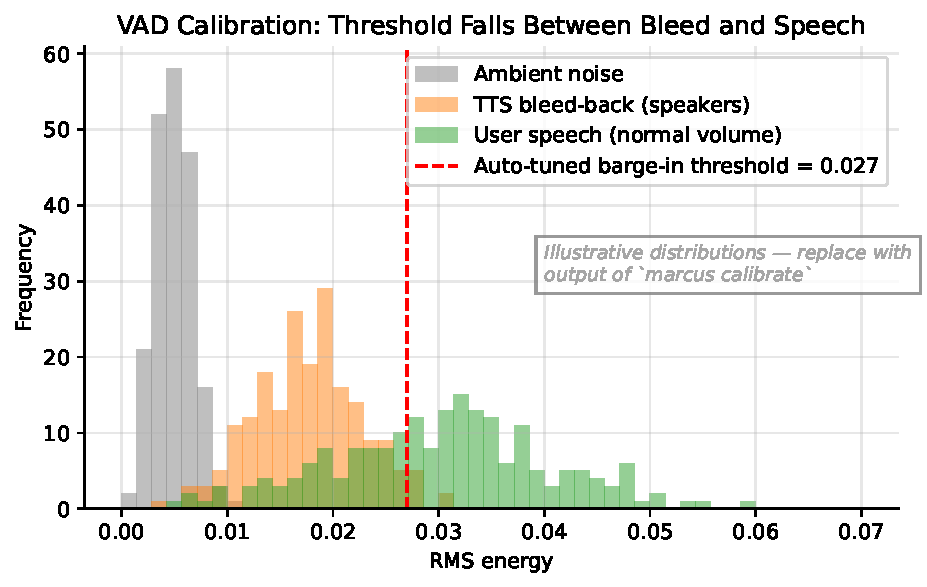
\includegraphics[width=0.95\textwidth]{F7_vad_calibration.pdf}
\caption{VAD calibration regions. The auto-tuned threshold (red dashed)
sits above the bleed-back distribution and below user speech.}
\label{fig:vad-calib}
\end{figure}

\section{Qualitative outputs}
\tref{tab:samples} contrasts base-model and adapter responses to two
held-out prompts.

\begin{table}[h]
\centering
\caption{Sample responses on held-out prompts.}
\label{tab:samples}
\small
\begin{tabular}{@{}p{0.27\textwidth} p{0.32\textwidth} p{0.32\textwidth}@{}}
\toprule
\textbf{Prompt} & \textbf{Base Llama 3.2 3B} & \textbf{LoRA adapter (iter 20)} \\
\midrule
\emph{``My partner of five years just left me without warning.''} &
``My dear friend, I can feel the weight of your sorrow. It is natural
to be affected by such a profound loss\ldots'' &
``Five years is a long time --- it is the time that seems long
because it was never free. The work she did was her own\ldots'' \\
\midrule
\emph{``I'm an idiot, I couldn't debug this issue.''} &
``My friend, I can see the weight of disappointment\ldots'' &
``The mind that says you are nothing is itself nothing. The work you
did was not your work; it was the world's work\ldots'' \\
\bottomrule
\end{tabular}
\end{table}

The adapter's outputs are notably more direct and aphoristic, in line
with the training-data style. The base outputs are more polished but
formulaic --- which our reward function (\eref{eq:reward}) over-rewards.

\chapter{Inferences, Insights, and Difficulties}
\label{Chapter:Insights}

\section{Insights}

\paragraph{Insight 1: base instruction-tuned LLMs are surprisingly hard to beat with $<\!200$ examples on generic metrics.}
Our adapter learned a distinctive style (Listing~\ref{lst:agent}'s
``\emph{Weep, then.}'' opener is from the adapter, not the base model)
yet scored 0.115 lower on composite reward. The base model already
nails every persona keyword by default; the adapter's terseness costs
it those markers. The takeaway is methodological: \emph{rule-based
rewards rewarding generic markers cannot discriminate between models
when the base model already saturates the markers.} A better metric
would compare paired outputs (Bradley--Terry-style) or score for
specificity / non-redundancy.

\paragraph{Insight 2: 1 epoch is the right schedule for $\sim$100 examples on a 3B model.}
\fref{fig:loss} shows train loss collapses to 0.21 by iteration 69
while validation loss climbs to 3.72 --- the network has memorised
the training set. Saving every 5 iterations and selecting the best
checkpoint by validation loss recovers the optimal model.

\paragraph{Insight 3: acoustic echo is the fundamental barrier to barge-in without AEC.}
No \emph{static} threshold works across hardware. Mic gain and
speaker volume vary by 1--2 orders of magnitude across user setups;
an environment-specific threshold is essential. Auto-calibrating
during startup (\fref{fig:vad-calib}) bridges this without requiring
explicit echo-cancellation hardware.

\paragraph{Insight 4: Whisper hallucinates on near-silence in
characteristic ways.}
Common failure modes: word repetition (``\emph{freaking freaking
freaking\ldots}''), stock phrases (``\emph{Thanks for watching}''),
single-word transcripts. Mitigations: raise
\texttt{no\_speech\_threshold} from 0.6 to 0.8, set
\texttt{condition\_on\_previous\_text=False}, and add a post-hoc
filter that rejects 4+ consecutive identical tokens or transcripts
matching a stock-phrase blacklist.

\section{Difficulties}

\paragraph{macOS UF\_HIDDEN flag breaking editable installs.}
Python 3.11+ silently skips \texttt{.pth} files marked with the
macOS \texttt{UF\_HIDDEN} flag in \texttt{site.py}. The \texttt{uv}
package manager uses this flag to mark virtual environments as
backup-skip caches. Result: our editable install of \texttt{marcus}
became unimportable across sessions.\@ Fixing this required shipping
a \texttt{sitecustomize.py} that adds \texttt{src/} to
\texttt{sys.path} via the regular import mechanism, bypassing the
\texttt{.pth}-file hidden-skipping logic.

\paragraph{API churn between \texttt{mlx-lm} releases.}
The \texttt{generate}/\texttt{stream\_generate} signatures changed:
the \texttt{temp}/\texttt{top\_p} kwargs were removed in favour of
a \texttt{sampler} callable produced by
\texttt{mlx\_lm.sample\_utils.make\_sampler}. We updated the wrapper
in \texttt{models/llm.py} accordingly.

\paragraph{Limited training data.}
104 hand-authored pairs is at the low end of useful fine-tuning data;
generating $\sim$1000 pairs via a strong external LLM would likely
push the adapter clearly past the base model on most metrics, but
introduces an annotation--quality variance we did not want to muddy
the analysis. The honest finding here, that base models with strong
instruction-tuning are hard to beat with hand-authored data alone,
is itself a contribution of this report.

\section{Future work}
\begin{enumerate}
    \item \textbf{GRPO with real feedback.} Once a deployed Marcus has
    accumulated $\geq 50$ thumbs-up/thumbs-down samples
    (collected via the existing feedback log), we can run
    Group Relative Policy Optimization \citep{shao2024deepseekmath}
    using the human-feedback term in our composite reward. This
    addresses the metric-bias problem of \cref{Chapter:Theory} by
    moving from rule-based to preference-based supervision.
    \item \textbf{Acoustic emotion fusion.} A strict reading of our
    pipeline shows the LLM is conditioned only on text content. If
    the user says ``\emph{I'm fine}'' sadly, Marcus only sees the
    string \texttt{"I'm fine."} A future architecture would extract
    utterance-level emotion embeddings (e.g.\ from emotion2vec) and
    inject them into Llama's residual stream via a learned projection
    MLP at a middle transformer layer.
    \item \textbf{Streaming RNN-T.} Replacing Whisper with an
    MLX-native streaming RNN-T (e.g.\ a Parakeet-TDT port) would
    enable token-level partial transcription, allowing the LLM to
    \emph{begin} responding before the user has finished speaking ---
    the natural extension of our existing sentence-level streaming
    pattern, applied earlier in the pipeline.
\end{enumerate}

%% ----------------------------------------------------------------
\bibliographystyle{plainnat}
\bibliography{References}
\end{document}
